\documentclass[notes]{subfiles}

\begin{document}
	\chapter{Derivatives}
	\addcontentsline{toc}{section}{2.1 - Derivatives and Rates of Change}
	\setcounter{section}{1}
	\fancyhead[RO,LE]{\bfseries \large\nameref{cs21}} 
	\fancyhead[LO,RE]{\bfseries \currentname}
	\fancyfoot[C]{{}}
	\fancyfoot[RO,LE]{\large \thepage}	%Footer on Right \thepage is pagenumber
	\fancyfoot[LO,RE]{\large Chapter 2.1}
	
\section*{Derivatives and Rates of Change}\label{cs21}
	\subsection*{Before Class}
	\addcontentsline{toc}{subsection}{Before Class}
	\subsubsection*{Tangents}
	\addcontentsline{toc}{subsubsection}{Tangents}
		\begin{question}
			How did we define the slope of the secant line between two points $(a,f(a))$ and $(x,f(x))$?
		\end{question}
			\vspace*{1in}

		\begin{defn}[Slope of the Tangent Line 1]
			The \textbf{tangent line} to a curve $y = f(x)$ at the point $P(a,f(a))$ is the line through the point $P$ with slope
			\showto{ins}{
				\[m = \lim_{x\to a} \dfrac{f(x)-f(a)}{x-a}\]
			}
			\showto{st}{
				\\ \vspace{.75in}
			}
			provided that this limit exists.
		\end{defn}
		Here are some pictures to help give some intution to the definition:

			\newpage
			
		\begin{ex}
			Find the slope of the tangent line through the points $(a,f(a)))$ and $(a+h,(f(a+h))$
		\end{ex}
			\vs{1}
			
		\begin{defn}[Slope of the Tangent Line 2]
			The \textbf{tangent line} to a curve $y = f(x)$ at the point $P(a,f(a))$ is the line through the point $P$ with slope
			\showto{ins}{
				\[m = \lim_{h\to 0} \dfrac{f(a+h)-f(a)}{h}\]
			}
			\showto{st}{
				\\ \vspace{.75in}
			}
			provided that this limit exists, where $h$ is considered to be a
			\showto{ins}{
				\fbox{small change in $x$}.
			}
			\showto{st}{
				\blank{2.2}.
			}
		\end{defn}
		Here are some more pictures for the new defintion:
			\vs{2}

			\newpage
		
	\subsubsection*{Tangents \& Velocities}
	\addcontentsline{toc}{subsubsection}{Tangents \& Velocities}	
		\begin{question}
			Rewrite what it means for a line to be \emph{tangent} to a curve, and what it means for a line to be \emph{secant} to a curve.
		\end{question}
			\vs{1}
				
		\begin{question}
			In \S1.4, we discussed how to compute average velocity$-$what was the formula?  How could we find instantaneous velocity from average velocity?
		\end{question}
			\vs{1}
			
		\begin{rmk}[Instantaneous Velocity]
			The \emph{instantaneous velocity} of an object, given its position function $f(x)$, is
			\showto{ins}{
				\[v(a) = \lim_{h\to 0} \dfrac{f(a+h)-f(a)}{h}\]
			}
			\showto{st}{
				\\ $ $\vspace{.55in} 
			}
		\end{rmk}
		\begin{ex}
			Suppose that a ball is dropped from the upper observation deck of a building which is 980 m above the ground.
			\begin{enumerate}[(a)]
				\item What is the velocity of the ball after 10 seconds?  Use that the equation of motion is $s(t) = 4.9t^2$.
					\vs{1}
				\item How fast is the ball traveling when it hits the ground?
					\vs{1}
			\end{enumerate}
		\end{ex}
			\newpage
	\subsubsection*{Derivatives}
	\addcontentsline{toc}{subsubsection}{Derivatives}
		\begin{defn}[The Derivative (at $x = a$)]
			The \textbf{derivative of a function} $f$ at input $x = a$ is given by
			\showto{ins}{
				\[f'(a) = \lim_{h\to 0} \dfrac{f(a+h)-f(a)}{h}\]
			}
			\showto{st}{
				\\ \vspace{.5in}
			}
			or
			\showto{ins}{
				\[f'(a) = \lim_{x\to a} \dfrac{f(x)-f(a)}{x-a}\]
			}
			\showto{st}{
				\\ \vspace{.5in}
			}
			if this limit exists.
		\end{defn}
			
		We have two ways of interpreting what the derivative actually means:
		\showto{ins}{
			\begin{itemize}
				\item The derivative $f'(a)$ is the \fbox{instantaneous rate of change of $y = f(x)$ with respect to $x$}\\ \fbox{when $x =a $}.
				\item The derivative $f'(a)$ is \fbox{equal to the slope of the tangent line to the function $y = f(x)$}\\ \fbox{at the point $(a,f(a))$}.
			\end{itemize}
		}
		\showto{st}{\\
			\begin{itemize}
			\setlength\itemsep{15pt}
				\item The derivative $f'(a)$ is the \blank{4.5}\\[15pt] \blank{4}.
				\item The derivative $f'(a)$ is \blank{5} \\[15pt] \blank{3}.
			\end{itemize}
		}	
		\begin{ex}
			Let $f(x) = x^2$.  Show that $f'(1) = 2$ using \emph{both} formulas for the derivative at a point.
		\end{ex}
			\newpage
		
	\subsubsection*{Pre-Class Activities}	
	\addcontentsline{toc}{subsubsection}{Pre-Class Activities}
		\begin{ex}
			We have two definitions of the derivative at a point, $x = a$.  Rewrite them here.
		\end{ex}
			\vs{1}
			
		\begin{ex}
			Let $f(x) = x^2 + 1$ and $a = 3$.
			\begin{enumerate}[(a)]
				\item Using either definition you wrote down above, complete the \emph{setup} for the derivative.  \textbf{Do not use algebra; that is what part (b) will do}.  You only need to write the setup. \\[20pt]
					\begin{minipage}{3in}
						\begin{flushright}
						\Large{$f'(x) = \lim$}
						\end{flushright}
					\end{minipage}
					\vs{.25}
				
				\item Simplify your answer from part (a) to show that $f'(3) = 6$.
					\vs{1.5}
			\end{enumerate}
		\end{ex}
		
		\begin{ex}
			A function $f(x)$ is graphed, along with several tangent lines.  Identify the derivative at the points $x = -3$ and $x = 2$
			\begin{flushleft}
				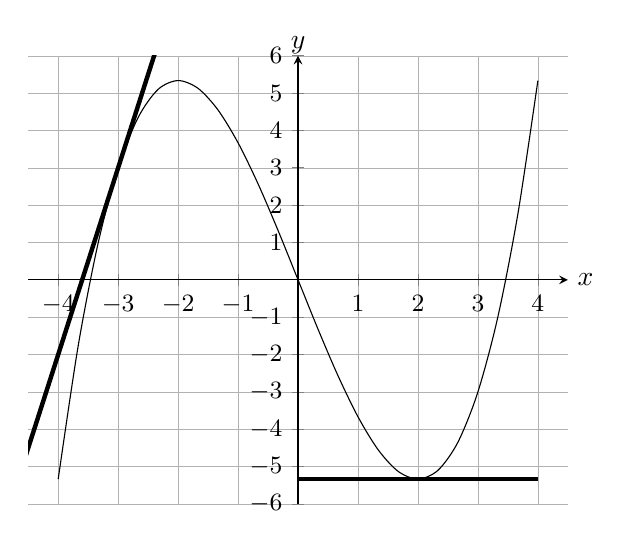
\begin{tikzpicture}
					\begin{axis}[
							grid style = {line width = .1pt, draw = gray!60},
							grid = both,
							every tick label/.append style={font=\small},
							axis x line = middle,
							axis y line = middle,
				    			every axis y label/.style={at={(ticklabel cs:1.15)}, yshift = -3pt},
								y label style={at={(axis description cs: 0.5, 1)},above},
							ytick = {-10,-9,-8,-7,-6,-5,-4,-3,-2,-1,1,2,3,4,5,6,7,8,9,10},
				    			ylabel = {$y$},
				    			ymin = -6, ymax = 6,
			    				every axis x label/.style= {at ={(ticklabel cs:1)}},
			    				xtick = {-4,-3,-2,-1,1,2,3,4},
				    				x label style={at={(axis description cs: 1, 0.5)},right},
			    				xlabel = {$x$},
			    				xmin = -4.5, xmax = 4.5			
						]
						\addplot[smooth,domain = -4:4] {(1/3)*x^3 - 4*x};
						\addplot[smooth, ultra thick, domain = 0:4] {-16/3};
						\addplot[smooth, ultra thick, domain = -6:0] {5*x + 18};
					\end{axis}
				\end{tikzpicture}
			\end{flushleft}
		\end{ex}
				\newpage
				
		\begin{ex}
			Imagine that a classmate couldn't watch the videos and didn't have the workbook for this section, and has asked you to explain the relationship between average rate of change, instantaneous rate of change, tangent lines, and secant lines.  What would you tell them?
		\end{ex}
			\vs{1} $ $
		\newsec
	\subsection*{In-Class}
	\addcontentsline{toc}{subsection}{In-Class}
		\begin{question}
			There are a few ways to write a line$-$what are they?
		\end{question}
			\vs{1}
			
		\begin{ex}
			\begin{enumerate}[(a)]
				\item Use both definitions of the derivative at a point to show that for $f(x) = x^3$, $f'(1) = 3$.
					\vs{1.5}
					
				\item Find the equation of the tangent line to $f(x)$ at the point $x = 1$.
					\vs{1}
					
			\end{enumerate}
		\end{ex}
			\newpage		
		\begin{ex}
			\begin{enumerate}[(a)]
				\item Use the first definition of the derivative to find $g'(2)$ for $g(x) = \dfrac{2}{x}$.
					\vs{1}
					
				\item Use the second definition of the derivative to find $g'\lrpar{\dfrac{1}{2}}$ for $g(x) = \dfrac{2}{x}$.
					\vs{1}
					
				\item Use either definition of the derivative to find $g'(10)$ for $g(x) = \dfrac{2}{x}$.
					\vs{1}
					
				\item Find the equation of the tangent line to $g(x)$ at $x = \dfrac{1}{2}$ and at $x = 10$.
					\vs{1}					
			\end{enumerate}  
		\end{ex}
			\newpage

		\begin{question}
			Do these slopes make sense given the graph of $g(x)$?  Make a conjecture about the slopes as $x$ gets arbitrarily large (as $x\to \infty$), and as $x\to 0^+$.
		\end{question}
			\vs{1}

		\begin{ex}
			Find the derivative of the function $f(x) = x^2-6x+1$ at the input $x = a$.
		\end{ex}
			\vs{2}
			
		\begin{ex}
			Find the equation of the tangent line to the parabola $y = x^2 + 4x$ at the point $(-1,-3)$.
		\end{ex}
			\vs{2}
			\newpage
			
		\begin{ex}
			Find an equation of the tangent line to the graph of $y = h(x)$ at $x = 5$ if $h(5) = -3$ and $h'(5) = 4$.
		\end{ex}
			\vs{1}
			
		\begin{ex}
			If $\ds f'(a) = \lim_{h\to 0} \dfrac{\sqrt{16 + h} - 4}{h}$ represents the derivative of the function $f(x)$ at $x = a$, what is $f(x)$ and what is $a$?
		\end{ex}
			\vs{1}
			
	\subsubsection*{Rates of Change}
	\addcontentsline{toc}{subsubsection}{Rates of Change}
		If we use the function $y = f(x)$, then the derivative tells us the rate of change of the \emph{output} $y$ with respect to the \emph{input} $x$.  Another way of writing this is
			\showto{ins}{
				\[\text{instantaneous ROC} = \lim_{\Delta x\to 0} \dfrac{\Delta y}{\Delta x} = \lim_{x_2\to x_1}\dfrac{f(x_2)-f(x_1)}{x_2-x_1}\]
			}
			\showto{st}{
				\vspace{1in}
			}
			
		\begin{ex}
			The function $C$ gives the number of bushels of corn produced on a tract of farmland that is treated with $f$ pounds of nitrogen per acre.
			\begin{enumerate}[(a)]
				\item Is it possible for $C(90)$ to be negative?  Why or why not?
					\vs{1}
					\newpage
					
				\item What are the units on $C'(90)$?
					\vs{.5}

				\item Is it possible for $C'(90)$ to be negative?  Why or why not?
					\vs{1}
			\end{enumerate}
		\end{ex}
			
		\begin{ex}
			The function $p$ gives the number of miles from an airport that a plane has flown after $t$ hours.
			\begin{enumerate}[(a)]
				\item What are the units of $p'(1.5)$?
					\vs{1}

				\item What is the common word used for $p'(1.5)$?
					\vs{1}
			\end{enumerate}
		\end{ex}

		\begin{ex}
			The cost of producing $x$ ounces of gold from a new gold mine is $C=f(x)$ dollars.
			\begin{enumerate}[(a)]
				\item What is the meaning of the derivative $f'(x)$?  What are its units?
					\vs{1}
				\item Interpret the statement $f'(800) = 17$.
					\vs{1}
			\end{enumerate}
		\end{ex}
			\newpage
			
	\subsection*{After Class}
	\addcontentsline{toc}{subsection}{After Class}
		\begin{ex}
			The tangent line to $y = f(x)$ at $(3,4)$ passes through the point $(0,2)$.  Find $f(3)$ and $f'(3)$.
		\end{ex}
			\vs{1}
			
		\begin{ex}
			Sketch the graph of a function $f$ for which $g(0) = g(2) = g(4) = 0$, $g'(1) = g'(3) = 0$, $g'(0) = g'(4) = 1$, $g'(2) = -1$, $\ds \lim_{x\to 5^-} g(x) = \infty$, and $\ds \lim_{x\to -1^+} g(x) = -\infty$.
		\end{ex}
			\vs{2}
			
		\begin{ex}
			$\ds \lim_{\theta\to \pi/6} \dfrac{\sin\theta - \frac{1}{2}}{\theta - \pi/6}$ represents the derivative of a function $f(\theta)$ at some value of $\theta = a $.  What is $f(\theta)$ and what is $a$?
		\end{ex}	
			\vs{1}
			
	\clearpage
\end{document}